\chapter{Fondamenti e stato dell'arte}
\label{sec:background}

% Source notes: Vault/wiki (concepts: Prefill and Decode, KV Cache, On-Device Inference, Apple Silicon and MLX, Energy of
% LLM Inference, decision model Models, Letter-Token Readout, Laya, Decision-Model Benchmarks, Groundedness Verification,
% Hallucination Detection, Calibration, Verbalised vs Logit Confidence, Fine-tuning Instability and Seeds).

Questo capitolo passa in rassegna i lavori su cui GroundOne si fonda e quelli con cui viene confrontato. Il costo
dell'inferenza su un dispositivo locale, da cui discende il progetto, è già stato trattato nel Capitolo~\ref{sec:local}.
Si parte dai decision model, cioè dall'idea di leggere le decisioni di un modello linguistico invece di farle
generare, e dal loro ecosistema, in rapida crescita. Seguono il problema delle allucinazioni nella
retrieval-augmented generation (RAG) e i metodi che verificano le risposte rispetto alle fonti. Il capitolo si chiude con
la calibrazione, con il parameter-efficient fine-tuning e con la lacuna che questa tesi intende colmare.

\section{Decision Model}
\label{sec:bg-systemone}

Il termine \emph{System One model} è stato introdotto da TypeSafe con Jev, un modello offerto come servizio remoto. Jev
risponde a domande chiuse su uno stato dato, cioè sul contesto fornito nella richiesta, e restituisce output tipizzati,
come un booleano, una scelta tra opzioni o un punteggio, senza generare testo~\cite{typesafe2026jev}. Il nome richiama il
pensiero veloce e intuitivo descritto da Kahneman, contrapposto al ragionamento deliberato. Il fornitore dichiara latenze
comprese tra le decine e le centinaia di millisecondi e forti risparmi rispetto ai giudici generativi. Queste cifre,
però, restano dichiarazioni del fornitore, e l'architettura non è resa pubblica.

Le implementazioni open arrivate in seguito si distinguono per il modo in cui producono le probabilità, e se ne possono
individuare tre famiglie. La più diffusa presenta la domanda come una scelta multipla e conserva la head del modello
linguistico, cioè lo strato finale che assegna un punteggio a ogni token del vocabolario: la decisione si legge dai
logit delle lettere delle opzioni, nella posizione in cui il modello scriverebbe la risposta. SemIf applica questo
readout a un modello da 4B parametri lasciato congelato, cioè senza modificarne i pesi, e riporta che 21 criteri relativi
a un documento ottengono risposta in circa un secondo; la migliore baseline generativa capace di produrre JSON valido
impiega invece più di cinque secondi~\cite{semif}. Rizzo-Flow, a differenza di SemIf, addestra con LoRA un modello da 4B
su decisioni tipizzate ed espone la stessa interfaccia di Jev. I suoi autori riportano che il fine-tuning ne migliora sia
l'accuratezza sia la calibrazione~\cite{rizzoflow}. È uno dei due decision model generalisti usati come baseline in questa tesi.

La seconda famiglia codifica separatamente lo stato e ciascuna risposta candidata, e ne confronta gli embedding, cioè i
vettori numerici che rappresentano ciascun testo. I Contrastive Language Models, che appartengono a questa famiglia, sono
molto veloci quando i candidati sono numerosi e riutilizzabili. Nel confronto riportato dagli stessi autori, però,
concordano con le decisioni di Jev molto meno di un modello che fa interagire stato e candidato~\cite{kwok2026clm}. La
terza famiglia usa piccoli encoder\footnote{Il \emph{token di maschera} è un token speciale che, durante il preaddestramento,
prende il posto delle parole che il modello deve ricostruire.} con una head decisionale dedicata. Laya, per esempio, si
basa su un encoder ModernBERT da circa 400M parametri e assegna un punteggio a ogni opzione in corrispondenza del relativo
token di maschera. Le domande di una richiesta sono valutate in un'unica chiamata, raggruppate in un batch, ma ciascuna
viene codificata insieme a una propria copia del contesto~\cite{convai2026laya,azizi2026labels}.

Le evidenze a supporto di questi sistemi sono disomogenee. La maggior parte proviene dagli autori stessi, spesso su una
sola macchina e su un solo benchmark. Le valutazioni indipendenti sono recenti e meno favorevoli ai piccoli modelli
open. Una valutazione di Jev su 37 dataset trova ben calibrate le probabilità che il modello assegna alle scelte fra
opzioni. Le probabilità binarie, invece, ordinano bene gli esempi ma risultano mal posizionate rispetto a una soglia
fissa di 0.5. Lo stesso studio riporta per Jev una balanced accuracy media di 78.6, espressa in percentuale, su LLM-AggreFact~\cite{deusser2026jev}. Una riproduzione indipendente di Laya osserva una calibrazione diversa da
quella dichiarata e una forte dipendenza da una temperatura di calibrazione stimata sui dati di
destinazione~\cite{nandakishore2026laya}. Un benchmark costruito su coppie contrastive, cioè su decisioni quasi identiche che differiscono per un solo
dettaglio decisivo, colloca i piccoli modelli open molto al di sotto di Jev~\cite{yong2026decidebench}. Infine, è stato mostrato che, quando l'etichetta di un'opzione e la
sua definizione sono in conflitto, i decision model tipizzati seguono l'etichetta anziché la
definizione~\cite{azizi2026labels}.

L'ecosistema, intanto, cresce rapidamente. Il 9 ottobre 2026 l'hub di Hugging Face ha introdotto ufficialmente un tag
dedicato a questi \emph{decision model}~\cite{hf2026decisionmodels}. Il giorno successivo il tag raccoglieva già circa
1500 modelli, pubblicati da circa 600 autori e di qualità molto variabile. Questa tesi usa il termine
\emph{decision model}, adottato dall'ecosistema; \emph{System One} resta il nome con cui TypeSafe ha introdotto la
categoria, e compare nel seguito soltanto come nome dell'interfaccia compatibile con Jev.

Poche settimane dopo il rilascio di Jev, anche organizzazioni affermate hanno pubblicato i propri decision model open.
Clef di Cloudflare aggiunge a un decoder una head decisionale dedicata e risponde a tutte le domande con un solo
forward pass sullo stato: è l'architettura che per Jev era stata soltanto ipotizzata~\cite{cloudflare2026clef}. d1-3B di
Liquid AI legge la decisione da un insieme ristretto di lettere di risposta, con un modello da 3B il cui stato è
condiviso da tutte le domande~\cite{liquid2026d1}. Perplexity, infine, applica il fine-tuning a un modello da 27B con una
head sulle lettere~\cite{perplexity2026decider}. Una leaderboard della comunità, il Decision Index, valuta questi modelli
su una batteria comune di benchmark pubblici, tra cui RAGTruth valutato a livello di risposta
intera~\cite{decisionindex2026}. I risultati tracciano una linea netta. I decision model generalisti con meno di un
miliardo di parametri superano a stento la baseline banale su RAGTruth, e soltanto i modelli da decine di miliardi di
parametri individuano in modo affidabile le risposte allucinate.

Gli studi su Jev aggiungono tre osservazioni. Le sue probabilità sono calibrate se aggregate su molti task, ma non sul
singolo task. Soglie e temperature vanno stimate sul carico di lavoro di destinazione~\cite{guo2026justaskjev,li2026jevjudge}.
Scegliere la soglia tramite un limite inferiore di confidenza, infine, rende più sicuro mettere in produzione un giudice
che restituisce soltanto decisioni~\cite{li2026jevjudge}. Anche i runtime si sono adeguati: llama.cpp supporta ora
nativamente l'interfaccia System One~\cite{llamacpp}. Nessuno di questi modelli, tuttavia, è specializzato nella
groundedness, cioè nell'aderenza della risposta al documento. Nessuno, inoltre, riporta risultati di verifica a tre classi
a livello di frase sui benchmark usati in questa tesi.

Il readout sulle lettere è stato studiato anche al di fuori della letteratura sui decision model, nelle domande a scelta
multipla. Qui si possono confrontare due modi di ottenere la risposta di un modello addestrato a seguire istruzioni
(instruction-tuned): leggere quale lettera ha la probabilità più alta come primo token, oppure lasciare che il modello
scriva la risposta per esteso. Le due risposte spesso non coincidono~\cite{wang2024myanswerc}. Il readout, inoltre,
privilegia particolari identificatori di opzione, come certe lettere, e questo bias si può stimare e
rimuovere~\cite{zheng2024mcq}. Entrambi i risultati riguardano modelli usati zero-shot. Suggeriscono che un readout sulle
lettere, se deve servire da decisione, vada addestrato, calibrato o entrambe le cose. Nessun decision model open, inoltre, è
stato specializzato nella verifica della groundedness e poi confrontato, in condizioni controllate e sullo stesso
hardware, con giudici generativi, con verificatori specializzati e con decision model generalisti, di cui uno della stessa
dimensione.

\section{Retrieval-augmented generation e allucinazioni}
\label{sec:bg-rag}

La retrieval-augmented generation (RAG) dà a un modello linguistico accesso a documenti su cui non è stato addestrato: un
retriever seleziona i passaggi pertinenti alla domanda e il modello scrive la risposta con questi passaggi nel
contesto~\cite{lewis2020rag}. È l'approccio standard per costruire assistenti su documenti privati e può girare
interamente su una macchina locale. Non elimina però le allucinazioni. Le rassegne della letteratura distinguono due tipi
di errore. Gli errori di \emph{fattualità} (factuality) si misurano rispetto alla conoscenza del mondo, quelli di
\emph{fedeltà} (faithfulness) rispetto all'input o al contesto forniti al modello~\cite{huang2025hallucination}. Una
risposta RAG, in particolare, può essere infedele proprio ai passaggi che ha ricevuto, contraddicendoli o aggiungendo
informazioni che essi non contengono.

RAGTruth documenta quanto ciò sia frequente. Il dataset raccoglie circa 18{,}000 risposte, scritte da sei modelli
linguistici in tre task di tipo RAG, e vi annota con precisione al carattere le porzioni di testo in conflitto con il
contesto o non supportate da esso~\cite{niu2024ragtruth}. La distinzione di RAGTruth tra contenuto in conflitto e
contenuto privo di fondamento corrisponde alle classi \emph{contraddetta} e \emph{non menzionata} adottate in questa
tesi.

\section{Verifica della groundedness}
\label{sec:bg-verification}

Verificare una risposta rispetto alla fonte è un problema strettamente legato alla natural language inference (NLI). Nella
NLI si stabilisce se una premessa implica un'ipotesi (entailment), la contraddice o è neutrale rispetto a essa. Grandi
dataset di NLI forniscono dati di addestramento: MultiNLI~\cite{williams2018mnli} e ANLI~\cite{nie2020anli}, quest'ultimo
costruito in modo avversariale, cioè raccogliendo esempi scritti apposta per ingannare i modelli del momento.
VitaminC~\cite{schuster2021vitaminc} aggiunge coppie contrastive, in cui una revisione minima di una frase di Wikipedia
ribalta il verdetto: il modello è così costretto a guardare al fatto preciso e non alla sovrapposizione di parole.

Applicare questi modelli a testi generati lunghi richiede di scomporli. SummaC suddivide in frasi sia il documento sia il
riassunto e aggrega i punteggi di inferenza calcolati frase per frase~\cite{laban2022summac}. FActScore, invece, scompone
le generazioni lunghe in fatti atomici e li verifica uno per uno~\cite{min2023factscore}. La verifica a livello di frase,
adottata da GroundOne, è una via di mezzo tra un unico punteggio per l'intera risposta e la scomposizione in fatti atomici. Le frasi sono le unità naturali di una risposta, l'utente può intervenire su
una frase segnalata e il numero di decisioni cresce con la lunghezza della risposta.

Nella pratica prevalgono due famiglie di verificatori. La prima è quella degli encoder specializzati, piccoli e veloci.
AlignScore addestra un'unica funzione di allineamento su un'ampia miscela di task~\cite{zha2023alignscore}. MiniCheck
addestra piccoli verificatori su dati sintetici, costruiti in modo da richiedere un ragionamento su più frasi, ed eguaglia
modelli molto più grandi sui benchmark di grounding~\cite{tang2024minicheck}. HHEM è un modello di valutazione delle
allucinazioni dello stesso tipo, rilasciato come modello open~\cite{vectara2024hhem}. Questi modelli valutano ogni coppia
documento--frase in modo indipendente e restituiscono un'unica probabilità di supporto.

La seconda famiglia usa un modello linguistico come giudice, secondo lo schema
LLM-as-a-judge\footnote{Nello schema \emph{LLM-as-a-judge} un modello linguistico riceve tramite prompt il testo da
valutare e i criteri di valutazione, e scrive il proprio giudizio, a volte preceduto da una motivazione.}~\cite{zheng2023judging}.
Su giudici di questo tipo si basano framework di valutazione per RAG come RAGAS~\cite{es2024ragas} e
ARES~\cite{saadfalcon2024ares}. Lynx addestra con fine-tuning un giudice dedicato al rilevamento delle
allucinazioni~\cite{ravi2024lynx}, mentre Self-RAG addestra il generatore stesso a emettere token di critica, cioè token
speciali con cui il modello valuta i passaggi recuperati e il proprio output~\cite{asai2024selfrag}. I giudici sono
flessibili, ma il loro costo cresce con la quantità di testo che scrivono. I modelli piccoli usati come giudici, inoltre,
violano spesso il formato di output richiesto. Per garantire una risposta che il parser sappia interpretare serve allora
un decoding vincolato da una grammatica, che a ogni passo ammette soltanto i token compatibili con il formato
richiesto~\cite{willard2023outlines}. Il benchmark di riferimento per entrambe le famiglie è LLM-AggreFact, che riunisce
undici dataset di grounding annotati manualmente e li riconduce a un protocollo binario
comune~\cite{tang2024minicheck,llmaggrefact}. La Figura~\ref{fig:bg-verifiers} mette a confronto le due famiglie con il decision model specialista studiato in questa tesi.

\begin{figure}[htbp]
\centering
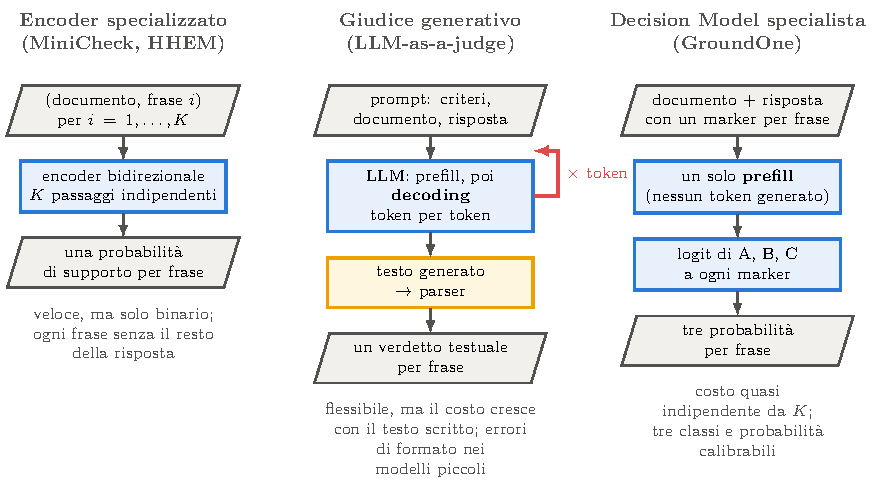
\includegraphics[width=\textwidth]{images/diagrams/bg_verifier_families_tikz.pdf}
\caption{Tre modi di verificare le $K$ frasi di una risposta. Un encoder specializzato valuta ogni coppia (documento, frase) in un forward pass separato e restituisce solo una probabilità di supporto. Un giudice generativo legge tutto, ma scrive il proprio verdetto token per token (ciclo rosso), quindi il costo cresce con il testo prodotto e l'output va interpretato da un parser. Un decision model specialista legge documento e risposta in un solo prefill e ricava da ogni marker tre probabilità, senza generare alcun token.}
\label{fig:bg-verifiers}
\end{figure}

\section{Calibrazione e selective prediction}
\label{sec:bg-calibration}

Una probabilità è calibrata quando, tra le predizioni fatte con una certa confidenza, la frazione di quelle corrette
coincide con tale confidenza: in un modello calibrato, per esempio, circa l'80\,\% delle predizioni fatte con confidenza
0.8 risulta corretto.
Le reti neurali moderne sono spesso mal calibrate, e una correzione semplice ed efficace è il temperature scaling: i
logit vengono divisi per un'unica costante, la temperatura\footnote{Con una temperatura $T > 1$ le probabilità diventano
meno estreme, con $T < 1$ più estreme. Poiché tutti i logit sono divisi per la stessa costante, la classe più probabile
non cambia.}, stimata su dati tenuti da parte~\cite{guo2017calibration}. La misura abituale della calibrazione è
l'Expected Calibration Error (ECE), che confronta confidenza e frequenza di predizioni corrette all'interno di fasce di
confidenza~\cite{naeini2015ece} (Sezione~\ref{sec:method-calibration}). Per i modelli linguistici interrogati tramite prompt può servire anche un bias per
classe, che corregga una preferenza sistematica verso alcune risposte~\cite{zhao2021calibrate}.

I modelli linguistici sanno, entro certi limiti, quello che sanno: sulle domande chiuse, le probabilità dei loro token
sono spesso informative sulla correttezza della risposta~\cite{kadavath2022know}. Quando le probabilità non sono
accessibili, si può chiedere al modello di esprimere la propria confidenza a parole. Nei modelli grandi sottoposti a
fine-tuning con feedback umano, questa confidenza verbalizzata può risultare calibrata meglio delle probabilità stimate
per campionamento~\cite{tian2023justask}. Valutazioni sistematiche, però, la trovano grossolana e troppo sicura, con
valori concentrati su pochi numeri tondi~\cite{xiong2024uncertainty}.

Una probabilità calibrata diventa utile grazie alla selective prediction: il sistema agisce sulle decisioni di cui è
sicuro e rinvia le altre. La curva risk--coverage descrive questo compromesso. Per ogni quota di decisioni accettate
(la coverage) riporta il tasso di errore su di esse (il risk), e mostra così come il tasso di errore scenda man mano che
si rinviano più decisioni~\cite{geifman2017selective}. La Figura~\ref{fig:bg-risk-coverage} ne illustra la forma tipica.

\begin{figure}[htbp]
\centering
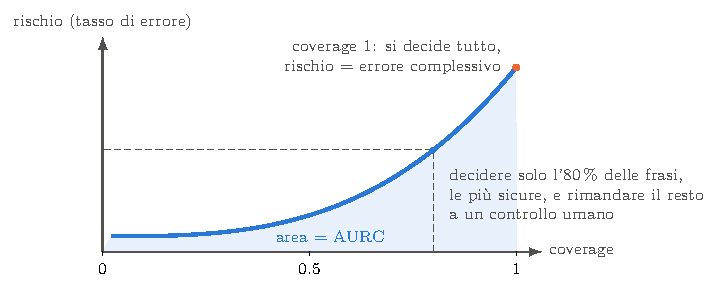
\includegraphics[width=0.75\textwidth]{images/diagrams/bg_risk_coverage_tikz.pdf}
\caption{Schema di una curva risk--coverage (forma illustrativa, non un risultato). Le decisioni sono ordinate dalla più sicura alla meno sicura; per ogni quota decisa (coverage) si riporta il tasso di errore (rischio) delle decisioni accettate. A coverage 1 il rischio coincide con l'errore complessivo; rinunciando alle decisioni meno sicure l'errore scende. L'area sotto la curva (AURC) riassume la curva in un numero: più è piccola, meglio la confidenza separa le decisioni corrette da quelle errate.}
\label{fig:bg-risk-coverage}
\end{figure}

\section{Parameter-efficient fine-tuning}
\label{sec:bg-peft}

Specializzare un modello preaddestrato non richiede di aggiornarne tutti i pesi. I metodi di parameter-efficient
fine-tuning (PEFT) addestrano soltanto una piccola quota di parametri e lasciano invariato il resto del modello. La
low-rank adaptation (LoRA) congela il modello e, per alcune matrici di pesi, addestra soltanto un aggiornamento a basso
rango\footnote{Il \emph{rango} di una matrice è il numero massimo di sue righe (o colonne) linearmente indipendenti. LoRA
impone che la correzione appresa per una matrice di pesi $d \times k$ abbia un rango $r$ piccolo. Una matrice di questo
tipo si può scrivere come prodotto di due matrici strette, una $d \times r$ e una $r \times k$, e basta quindi
memorizzare e addestrare queste due: $r(d+k)$ parametri invece dei $dk$ della matrice completa. In GroundOne 3B, per
esempio, una matrice $2048 \times 2048$ ha circa 4.2 milioni di pesi, mentre la sua correzione di rango 16 ne richiede
circa 65 mila, l'1.6\,\%.}. Al termine dell'addestramento, l'aggiornamento si può fondere nei pesi oppure mantenere come piccolo adapter
separato~\cite{hu2022lora}. Applicare LoRA a tutti gli strati lineari conta più che usare un rango elevato, e la tecnica
si combina con pesi di base quantizzati, così che anche modelli grandi stiano in poca memoria~\cite{dettmers2023qlora}.
La famiglia Qwen2.5 offre modelli open a partire da 0.5B parametri con un tokenizer condiviso, e permette quindi di
confrontare dimensioni diverse con la stessa ricetta~\cite{qwen2024qwen25}. La Figura~\ref{fig:bg-lora} schematizza un adapter LoRA applicato a uno strato lineare.

\begin{figure}[htbp]
\centering
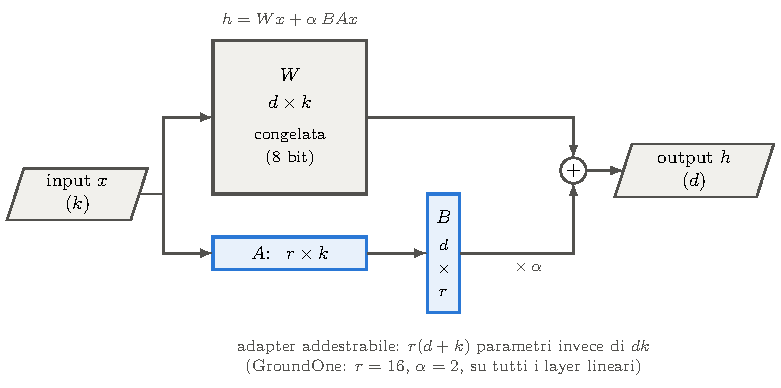
\includegraphics[width=0.8\textwidth]{images/diagrams/bg_lora_tikz.pdf}
\caption{Low-rank adaptation applicata a uno strato lineare. La matrice dei pesi $W$ resta congelata (in GroundOne a 8 bit); si addestrano soltanto le due matrici piccole $A$ e $B$, il cui prodotto, scalato di $\alpha$, si somma all'output dello strato. Con rango $r$ l'adapter ha $r(d+k)$ parametri invece dei $dk$ di $W$.}
\label{fig:bg-lora}
\end{figure}

Il fine-tuning su dataset piccoli, però, è notoriamente instabile. I risultati variano con il seed casuale, che determina
sia l'inizializzazione dei nuovi parametri sia l'ordine dei dati di addestramento~\cite{dodge2020finetuning}. Alcuni
addestramenti falliscono del tutto, e questo comportamento è legato a dettagli dell'ottimizzazione come l'assenza della
bias correction in Adam\footnote{Adam è un ottimizzatore che aggiorna ogni peso usando due medie mobili, una del
gradiente e una del suo quadrato, dette stime dei momenti. Poiché queste medie partono da zero, nei primi passi
sottostimano i valori veri; la \emph{bias correction} le riscala per compensare. AdamW è la variante di Adam che applica
il weight decay separatamente dal gradiente.}~\cite{mosbach2021stability}. Il gradient clipping, che limita la norma del
gradiente, è infine la difesa standard contro occasionali aggiornamenti esplosivi~\cite{pascanu2013difficulty}.

\section{Lacuna nella letteratura}
\label{sec:bg-gap}

Gli elementi necessari a un verificatore locale, veloce e calibrato esistono già, ma separatamente: modelli open
compatti e runtime che li eseguono su un laptop, l'idea dei decision model di leggere le decisioni anziché generarle,
verificatori specializzati e calibrazione post-hoc. Manca uno studio indipendente e controllato che li metta insieme su un
unico task. In particolare, nessun lavoro ha misurato se un decision model compatto, specializzato nella verifica della
groundedness, possa eguagliare su questo task i giudici generativi e gli encoder dedicati. Non è noto nemmeno da dove
provenga il suo vantaggio: dalla specializzazione, dal readout o dalla dimensione del modello. Resta infine da
stabilire se le sue probabilità siano abbastanza buone da fissare soglie e rinviare decisioni, e come il suo tempo e la
sua energia si confrontino con quelli di un giudice sullo stesso hardware consumer. Il resto della tesi affronta queste
domande.
